% arara: pdflatex
%        File: ComplexAnalysis.tex
%     Created: Sat Jun 24 03:00 PM 2023 B
% Last Change: Sat Jun 24 03:00 PM 2023 B
%
\documentclass[a4paper, 12pt]{article}
\usepackage[]{amsmath}
\usepackage{amsthm}
\usepackage{amssymb}
\usepackage{mathtools}
\usepackage{soul}
\usepackage[]{graphicx}
\graphicspath{ {./images/} }
\usepackage{caption}
\usepackage{subcaption}
\usepackage{hyperref}

\newtheorem{theorem}{Theorem}
\theoremstyle{definition}
\newtheorem{definition}{Definition}
\newtheorem{exercise}{Exercise}
\newtheorem{example}{Example}
\newtheorem{remark}{Remark}

\numberwithin{theorem}{section}
\numberwithin{definition}{section}
\numberwithin{exercise}{section}
\numberwithin{remark}{section}
\numberwithin{figure}{section}
\numberwithin{example}{section}

\newcommand{\R}{\mathbb{R}}
\newcommand{\C}{\mathbb{C}}
\newcommand{\intd}{\,\text{d}}

\renewcommand{\labelitemi}{$\circ$}
\renewcommand{\labelitemii}{*}

\DeclareMathOperator{\res}{Res}

\title{Complex Analysis Summary}
\author{Paul Joo-Hyun Kim}
\begin{document}
\maketitle
\tableofcontents
\setcounter{section}{-1}
\section{Preface}
This note is for people studying complex analysis,
and got lost in the middle with bunch of technical explanations.
I wil try my best to be succinct as possible,
stating important results (mostly without proof, but a bit of justification).

\textbf{Warning}: This summary note is not a substitute for the lecture note.
Make sure you study from lecture note!

\section{Complex Plane and M\"obius Maps}
\subsection{Complex Plane and Complex Infinity}
We will be working in what's known as the \textit{extended complex plane}.
Define the symbol $\C_{\infty} \coloneqq \C \cup \left\{ \underbrace{\infty}_{\text{Complex Infinity}} \right\}$;
that is, I refer to the space of complex numbers
and infinity.

Note that in $\C_{\infty}$, $\infty$ is different from infinity in real numbers.
$\infty \coloneqq \frac{1}{0}$ is a value that is not ``larger'' or ``smaller'' than any number
(since we are talking about complex number\dots), but rather
a number on a complex plane at a really far distance from origin.

It is \textbf{WRONG} to say:
\begin{itemize}
    \item $\infty \geq a$ for any $a \in \C_{\infty}$
    \item $\infty \leq a$ for any $a \in \C_{\infty}$
\end{itemize}
However, it is \textbf{CORRECT}\footnote{
    Subtlety here: it seems a bit dodgy to say $\infty = \infty$,
    but this is matter of definition;
    you won't really encounter this type of ``philosophical'' problem
    in your exam.
} to say:
\begin{itemize}
    \item $|\infty| \geq |a|$ for any $a \in \C_{\infty}$.
\end{itemize}
$\infty$ is not like a point on $\C$, but rather like a gigantic circle that you can never reach.

\subsection{M\"obius Maps}
\begin{definition}[M\"obius Map]
    $\psi : \C_{\infty} \rightarrow \C_{\infty}$ is a \textbf{M\"obius map} if:
    \begin{equation*}
        \psi \left( z \right) \coloneqq \frac{az + b}{cz + d}
    \end{equation*}
    where $
    \begin{pmatrix}
        a & b \\ c & d
    \end{pmatrix}
    $ is a nonsingular matrix.
    (This restriction removes the possibility of $\frac{0}{0}$,
    or trivial maps (eg: Constant function).)

    One needs to be careful when defining this function at infinity,
    but it should be sensible.\footnote{
    That said, if you are supposed to define what a M\"obius map is,
    you are \textbf{required} to definitions involving infinity as well.
    }
\end{definition}
\begin{exercise}[Composition of two M\"obius map is a M\"obius map]
    Show that for two M\"obius maps $\psi_1, \psi_2$,
    its composition $\psi_1 \circ \psi_2$ is also a M\"obius map.
\end{exercise}
\begin{remark}
    Consider the $2 \times 2$-matrix-to-M\"obius-map map as follows:
    \begin{equation*}
        f (A) \coloneqq
        \begin{pmatrix}
            a_{11} & a_{12} \\ a_{21} & a_{22}
        \end{pmatrix}
        \mapsto
        \frac{a_{11} z + a_{12}}{a_{21} z + a_{22}}
    \end{equation*}
    Then it turns out that
    $f\left( AB \right) = f(A) f(B)$
\end{remark}
\begin{exercise}[Decomposition of M\"obius maps]
    It turns out that M\"obius maps can be written as composition of
    \begin{itemize}
        \item translation
        \item dialation (``scaling by nonzero constant'')
        \item inversion ($z \mapsto \frac{1}{z}$)
    \end{itemize}
    Prove this. (Hint: You can do a constructive proof.)
\end{exercise}
M\"obius maps also has a very convenient property:
\begin{exercise}[Circline to Circline]
    Show that M\"obius maps map circlines to circline.
    (This means a line will either map to a circle or a line,
    and also a circle will either map to a circle or a line.)

    (Note: This is a boring long tedious proof, that probably won't be asked in exam,
    but don't take my word for it.)
\end{exercise}

\section{Complex Differentiability}
Complex differentiability is one of the highlights of the complex analysis.
\begin{definition}[Differentiable Function AKA Holomorphic Function]
    Take $a \in \C$.
    Let $f:U \rightarrow \C$ be a function where $U$ is a neighbourhood\footnote{Some open set containing $a$.} of $a$.
    Then $f$ is \textbf{(complex) differentiable} or \textbf{holomorphic} at $a$ if
    \begin{equation*}
        f'(a) = \lim_{z \rightarrow a} \frac{f(z) - f(a)}{z - a}
    \end{equation*}
    exists, and call it derivative of $f$ at $a$.
    If $f$ is differentiable for all points in $U$, then it is said to be
    differentiable/holomorphic on $U$.
\end{definition}
\begin{remark}
    Note that the definition seems to be have trivially extended from real analysis.
    \ul{However, there is a subtlety}.
    The limit does not approach just from positive or negative side,
    but from any direction. (Figure \ref{fig: Real and Complex Limit})
    \begin{figure}[tbp]
        \centering
        \begin{subfigure}[b]{0.5\textwidth}
            \centering
            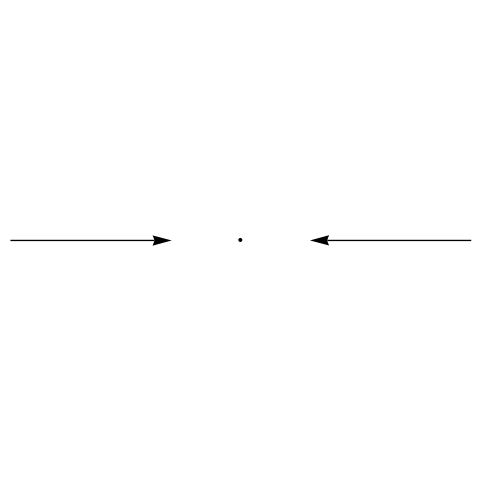
\includegraphics[width=\textwidth]{realLimit}
            \caption{Real Limit}
        \end{subfigure}
        \hfill
        \begin{subfigure}[b]{0.5\textwidth}
            \centering
            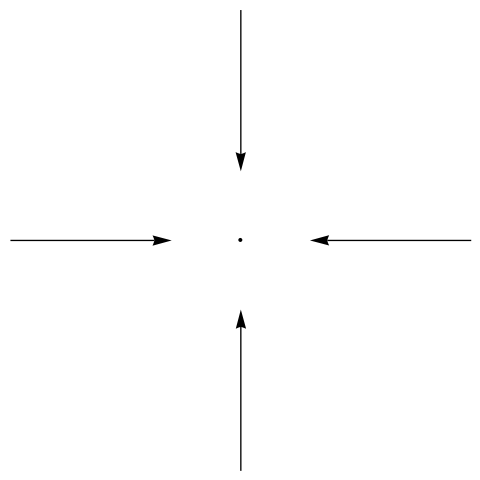
\includegraphics[width=\textwidth]{complexLimit}
            \caption{Complex Limit}
        \end{subfigure}
        \caption{Real limit (former) only concerns the approaching value from left and right side, but complex limit (latter) oncerns the approaching value from all direction.}
        \label{fig: Real and Complex Limit}
    \end{figure}
\end{remark}
\begin{exercise}[Differentiation Rules]
    Show that all differentiation rules from real analysis holds
    with holomorphic functions.
    \begin{itemize}
        \item Sum
        \item Product Rule
        \item Quotient Rule
        \item Chain Rule
    \end{itemize}
\end{exercise}
Due to the definition of complex limits being more restrictive,
a more nontrivial result follows.
\begin{exercise}[Cauchy-Riemann Equations]
    Let $a \in \C$ and $U$ be a neighbourhood of $a$.
    $f : U \rightarrow \C$ be holomorphic $a$.
    Write $f(z) = u(x,y) + i v(x,y)$ where $u,v$ are real functions
    and $z = x + iy$ where $x,y \in \R$.
    Then $\partial_x u, \partial_y u, \partial_x v, \partial_y v$ all exist,
    and the following \textbf{Cauchy-Riemann equations} hold:
    \begin{align*}
        \partial_x u &= \partial_y v \\
        \partial_x v &= - \partial_y u
    \end{align*}
(Hint: Figure \ref{fig: Real and Complex Limit} might give you an insight.)
\end{exercise}
\begin{remark}
    If Cauchy-Riemann does not hold, then it must mean that $f$ is not holomorphic! (Consider $f(z) = \bar{z}$. Cauchy-Riemann does not hold for any point, so it is nowhere holomorphic.)
\end{remark}
\begin{exercise}
    If $f(z) = u(x,y) + i v(x,y)$ is holomorphic on $U$,
    and $u,v$ are twice differentiable,
    deduce that $u$ and $v$ are \textit{harmonic}, that is,
    they satisfy the Laplace equation $\Delta u = \Delta v = 0$.
\end{exercise}
\begin{remark}
    It turns out complex plane reveals a lot about solving Laplace equation!
\end{remark}
Here is another kicker:
\begin{exercise}[Cauchy-Riemann to Holomorphic]
    If the partial derivatives exist and are continuously differentiable,
    Cauchy-Riemann implies holomorphicity.
\end{exercise}
\begin{remark}
    This means if you check that Cauchy-Riemann holds, you can immediately assume you can construct an analytic function!
\end{remark}
Holomorphic functions also have Taylor expansion:
\begin{remark}[Holomorphic functions have Taylor expansion]
    If $f$ is holormorphic at $a$, then
    in a neighbourhood of $a$, you can write
    \begin{equation*}
        f(z) = \sum_{n=0}^{\infty} c_n \left( z-a \right)^n
    \end{equation*}
    All the formulae for Taylor expansion holds (term-by-term differentiation, etc.)
\end{remark}
\begin{example}[Common Function Definitions]
    Here are definitions for some of the functions.
    \begin{align*}
        e^z = \exp z &\coloneqq \sum_{n=0}^{\infty} \frac{z^n}{n!} \\
        \cos{z} &\coloneqq \sum_{n=0}^{\infty} \left( -1 \right)^n \frac{z^{2n}}{\left( 2n \right)!} \\
        \cos{z} &\coloneqq \sum_{n=0}^{\infty} \left( -1 \right)^n \frac{z^{2n+1}}{\left( 2n + 1\right)!}
    \end{align*}
\end{example}
\begin{exercise}
    Show that
    \begin{align*}
        \cos{z} &= \frac{e^{iz} + e^{-iz}}{2} \\
        \sin{z} &= \frac{e^{iz} - e^{-iz}}{2i}
    \end{align*}
\end{exercise}
\begin{exercise}
    Show that $\exp \left( z+w \right) = \exp (z) \exp (w)$
\end{exercise}
\section{Branch Cut}
Sometimes, there is just no sensible way to define a function that it is holomorphic everywhere\dots
Two of the unfortunate (or fortunate) functions is the logarithm and square root.
We will first introduce the logarithm function.

Define logarithm function as:
\begin{equation*}
    \log z \coloneqq \log |z| + i \theta
\end{equation*}
where $\theta$ is the argument of $z$.

\begin{exercise}
    Verify that $\exp \left( \log z \right) = z$.
\end{exercise}

The choice of the interval for $\theta$ changes the behaviour of $\log z$ function.
For example, one could take the interval to be $\left[ 0, 2\pi \right)$,
or one could take it to be $\left[ - \pi, \pi \right)$,
or even just $\left[a, a + 2\pi\right)$ for some $a \in \R$.

The problem is that for given $z$, the argument of $z$ is not unique,
and if you try to define it continuously around a circle,
you will find that it is not possible\dots
(Figure \ref{fig: arg z multivalued}).
This means there needs to be some sort of contour from 0 that the function is not continuous on.
This is known as a \textbf{branch cut}, and you have total freedom to choose
based on what problem you want to solve.

\begin{figure}[tbp]
    \centering
    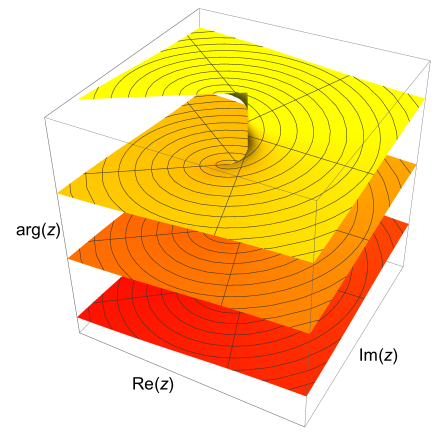
\includegraphics[scale=0.5]{argz}
    \caption{$\arg z$ being multivalued results in the need to introduce branch cut for logarithm.}
    \label{fig: arg z multivalued}
\end{figure}

\begin{example}[Where do we use branch cut?]
If you want to solve a problem with a fracture in an elastic solid (Figure \ref{fig: Crack Tip}),
one standard way to solve it is to find some holomorphic function outside of the crack $\left[ -c,c \right]$
satisfying some condition.
\begin{figure}[tbp]
    \centering
    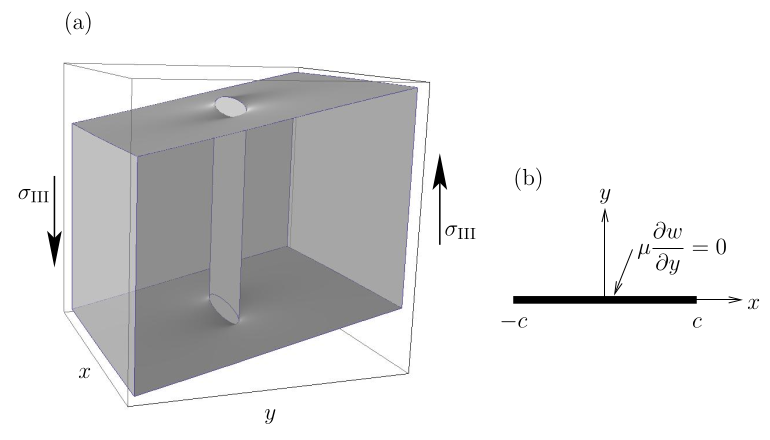
\includegraphics[scale=.5]{crackTip}
    \caption{Fracture in elastic material.}
    \label{fig: Crack Tip}
\end{figure}
It turns out that there is no function that is holomorphic everywhere satisfying that,
so you would define a ``branch cut'' to be the straight line $\left[ -c,c \right]$ to resolve it.
Then it is possible to define a function that is continuous away from the crack.
\end{example}

\begin{remark}
    When I say I am defining a branch cut,
    it means I am defining the function to be continuous away from the branch cut.
    I state this again due to its importance: \textbf{I am defining a function}.
\end{remark}

Branch cuts are something that honestly makes more sense once you \textbf{played around with it for a while}.

\begin{example}[Logarithm: branch cut along positive real axis]
    See Figure \ref{fig: Log Positive Real} for the diagram of a branch cut along positive real axis.
    $\log z \coloneqq \log |z| + \theta i$ where $\theta \in \left[ 0, 2\pi \right)$ has a branch cut along positive real axis.
    Right above the positive real axis, $\theta$ takes the value 0, so $\left(\log x\right)_{+} = \log |x|$.
    On the other hand, right below the positive real axis, $\theta$ takes the value $2\pi$, so $\left( \log x \right)_{-} = \log |x| + 2\pi i$

    So you might ask: \textit{What is $\log z$ where $z \in \R^{>0}$?} and the answer is,
    you are asking the wrong question, because we can only define the ``limiting value'' on each side of the branch cut,
    NOT on the branch cut.
    \begin{figure}[tbp]
        \centering
        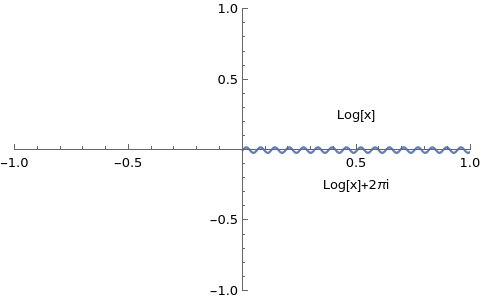
\includegraphics{logpositivereal}
        \caption{Logarithm function with branch cut along the positive real axis}
        \label{fig: Log Positive Real}
    \end{figure}
\end{example}
\begin{example}[Logarithm: branch cut along positive real axis]
    See Figure \ref{fig: Log Positive Imaginary}.
    This time take $\theta \in \left[ -\pi, \pi \right)$.
    On the right side of the branch cut, we have $\theta = \pi$, so
    $\left( \log \left( yi \right) \right)_{+} = \log{y} + \pi i$,
    whereas on the left side, we have $\theta = -\pi$, so
    $\left( \log \left( yi \right) \right)_{-} = \log{y} - \pi i$.

    \begin{figure}[tbp]
        \centering
        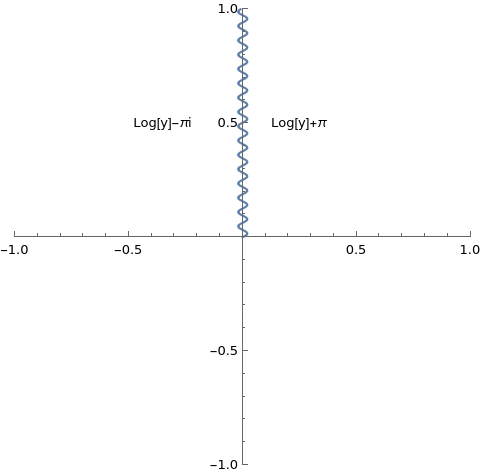
\includegraphics{logpositiveimaginary}
        \caption{Logarithm function with branch cut along the positive imaginary axis \textbf{Edit:} $\pi$ on the right side should be $\pi i$}
        \label{fig: Log Positive Imaginary}
    \end{figure}
\end{example}

\begin{exercise}[Square Root]
    Consider the definition of square root as given:
    \begin{equation*}
        z^{1/2} \coloneqq |z|^{1/2} e^{i \theta / 2}
    \end{equation*}
    (Note that I've just taken ``half'' as exponent in the polar form.)

    Define the branch cut along the negative real axis and evaluate $i^{1/2}$ in this branch.
    Define the branch cut along the negative imaginary axis and evaluate it again.
\end{exercise}
\begin{remark}
    In both square roots and logarithms, there was a point which the branch cut naturally starts from.
    These points are called \textbf{branch point};
    these are the points that you cannot avoid having a branch cut.
\end{remark}
\begin{remark}
    There is absolutely no need for a branch cut to be a straight line,
    and in some cases, it is more natural to define the branch cut in some other way (out of scope, however)
    Figure \ref{fig: spiral} is a classic example of non-straight branch.
    \begin{figure}[tbp]
        \centering
        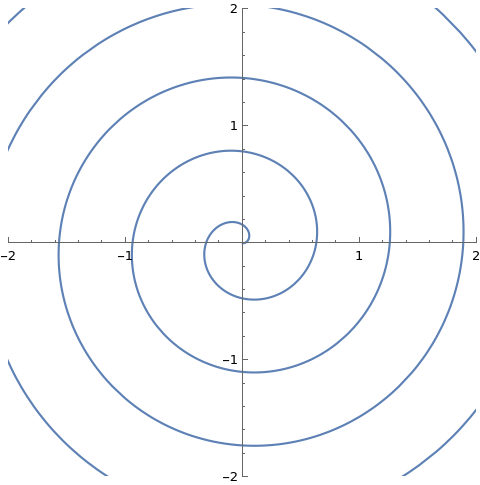
\includegraphics[scale=0.6]{spiral}
        \caption{A possible branch from a branch point (taken to be origin); a bit more complicated to describe, and often times, drawing this diagram might just be sufficient.}
        \label{fig: spiral}
    \end{figure}
\end{remark}
\begin{exercise}
    Try defining some branch cuts of $\left( 1+z \right)^{1/2}$.
    What is the branch point in this case?
\end{exercise}
\begin{example}[Square Root Branch Cut of Elastic Crack]
    \label{eg: Square Root Branch Cut of Elastic Crack}
    Suppose you want to define the branch of the function $\left( z^2 - 1 \right)^{1/2}$
    such that it is holomorphic away from the branch cut $\left[ -1,1 \right]$.

    Consider writing the function in a following way:
    \begin{equation*}
        \left( z^2 - 1 \right)^{1/2} = \left( z-1 \right)^{1/2} \left( z+1 \right)^{1/2}
    \end{equation*}
    Now note that $\left( z-1 \right)^{1/2}$ and $\left( z+1 \right)^{1/2}$ need branch cuts.
    One way to define them is through:
    \begin{align*}
        \left( z-1 \right)^{1/2} &= r_1^{1/2} e^{i\theta_1 / 2} \\
        \left( z+1 \right)^{1/2} &= r_2^{1/2} e^{i\theta_2 / 2}
    \end{align*}
    where $\theta_1, \theta_2 \in \left[ -\pi, \pi \right)$ (See Figure \ref{fig: Crack Tip 2}\footnote{
            The angle range is not a mistake, even though it might seem a bit unintuitive.
    })
    \begin{figure}[tbp]
        \centering
        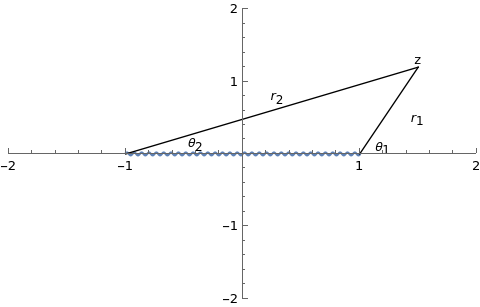
\includegraphics{crackTip2}
        \caption{$r_1, r_2, \theta_1, \theta_2$ as shown. The point on the upper right is the $z$. Branch cut is at $[-1,1]$.}
        \label{fig: Crack Tip 2}
    \end{figure}
    Hence, we get our branch cut between -1 and 1:
    \begin{equation*}
        \left( z^2 - 1 \right)^{1/2} = r_1^{1/2} r_2^{1/2} e^{i \left( \frac{\theta_1 + \theta_2}{2} \right)}
    \end{equation*}
\end{example}
\begin{exercise}
    Show that the branch cut defined on Example \ref{eg: Square Root Branch Cut of Elastic Crack}
    has different limiting values across the branch cut.
    \textbf{Again, the angle range given is not a mistake!}
\end{exercise}
\begin{exercise}
    Suppose the angle ranges are given to be $\theta_1 \in \left[ 0, 2\pi \right)$, $\theta_2 \in \left[ -\pi, \pi \right)$.
    Verify that the branch cuts are $(-\infty, -1] \cup [1, \infty) \subset \R$;
    that is, $\left( z^2 - 1 \right)^{1/2}$ has jump discontinuity across
    those intervals.

    (Hint: Sketch of the branch cut diagram is given as Figure \ref{fig: Crack Tip Out})
    \begin{figure}[tbp]
        \centering
        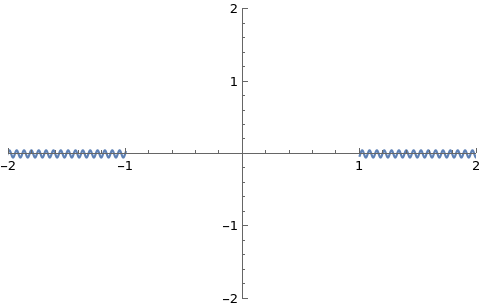
\includegraphics[scale=0.7]{crackTipOut}
        \caption{Branch cut diagram for $\theta_1 \in \left[ 0, 2\pi \right)$ and $\theta_2 \in \left[ -\pi, \pi \right)$}
        \label{fig: Crack Tip Out}
    \end{figure}
\end{exercise}
\begin{exercise}
    Let $f(z) = \left( k-i \right)^{1/2}$ with the branch cut at $i \left[ 1, \infty \right)$ (positive imaginary axis starting from $i$, the branch point).
    Show that $f(0) = e^{-i \pi/4}$.
\end{exercise}


\section{Paths and Integration}
You may have seen paths (AKA curves or lines) and integral along them
in multivariable calculus.
The complex analysis version is similar, but from a different perspective.
\subsection{Paths}
\begin{definition}[Path]
    Let $a < b$.
    $\gamma:[a,b] \rightarrow \C$ is a \textbf{path} if it is a continuous function.
    It is \textbf{closed} if $\gamma(a) = \gamma(b)$, that is, if the endpoints coincide.
\end{definition}
Tangent vector of a curve was an important concept in curves in MVC.
Similarly, one could define the notion of it in complex analysis by
introducing the ``derivative''.
\begin{definition}[Differentiability of Path]
    Path $\gamma:\left[ a,b \right] \rightarrow \C$ is \textbf{differentiable} at $t_0$ if
    its real and imaginary parts are differentiable at $t_0$,
    which is equivalent to saying
    \begin{equation*}
        \lim_{t \rightarrow t_0} \frac{\gamma(t) - \gamma(t_0)}{t-t_0}
    \end{equation*}
    exists.
    If so, we write this limit as $\gamma'(t_0)$.

    If $\gamma'(t)$ is continuous, then we say the path is in $C^1$.
\end{definition}
\begin{exercise}[``Tangent'']
    Show that $\gamma'(t)$ (if it exists) characterizes the tangent direction of the path $\gamma$.
    (Hint: Turn it into an MVC problem!)
    Explain what happens at $t_0$ if $\gamma'(t_0) = 0$.
\end{exercise}
\begin{example}
    \begin{figure}[tbp]
        \centering
        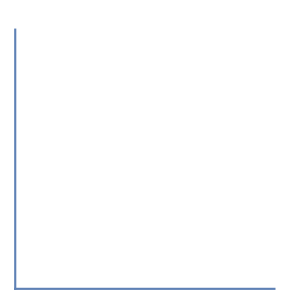
\includegraphics{pathRightAngle}
        \caption{Path given by piecewise $C^1$ path.}
        \label{fig: Path Right Angle}
    \end{figure}
    Consider
    \begin{equation*}
        \gamma(t) \coloneqq
        \begin{cases}
            t^2 &-1 \leq t \leq 0 \\
            it^2& 0 \leq t \leq 1
        \end{cases}
    \end{equation*}
    This is a piecewise $C^1$ path. See Figure \ref{fig: Path Right Angle}
    Note that $\gamma'(0) = 0$, so there is no ``tangent'' at the sharp corner.
\end{example}
\begin{example}[Circle]
    \textbf{One of the most important paths!}
    You can parameterize a circle with center $z_0$ and radius $r$ by:
    \begin{equation*}
        \gamma(t) = z_0 + r e^{it}
    \end{equation*}
    where $t \in \left[ 0, 2\pi \right]$.
    (You could also do $\gamma(t) = z_0 + r e^{2\pi i t}$ where $t \in \left[ 0, 1 \right]$)
    
    Note that the direction is counterclockwise.
\end{example}

\subsection{Complex Path Integral}
\begin{definition}[Complex Integral]
Given a complex function $F(t) = x (t) + i y(t)$,
one could define the integral over $t\in \left[ a,b \right]$ to be
\begin{equation*}
    \int_{a}^b F(t) \intd t \coloneqq \int_a^b x(t) \intd t + i \int_a^b y(t) \intd t
\end{equation*}
\end{definition}
\begin{exercise}
    Prove that, just like in real analysis, you can bound by the integral of the modulus of integrand; that is:
    \begin{equation*}
        \left| \int_a^b F(t) \intd t \right| \leq \int_a^b \left| F(t) \right| \intd t
    \end{equation*}
\end{exercise}
\begin{definition}[Path Integral]
    Given piecewise $C^1$ path $\gamma:[a,b] \rightarrow \C$ and $f: \C \rightarrow \C$, then
    \begin{equation*}
        \int_{\gamma} f(z) \intd z \coloneqq \int_{a}^b f\left( \gamma(t) \right) \gamma'(t) \intd t
    \end{equation*}
\end{definition}
\begin{remark}
    For remembering the definition,
    you can treat it as substitution rule in real integral:
    \begin{align*}
        z &= \gamma(t) \\
        \intd z &= \gamma'(t) \intd t
    \end{align*}
\end{remark}
\begin{example}[Terms in Taylor Around a Circle\footnote{Come back to this after you do residue theorem as well!}]
    \label{eg: Taylor Term Circle Integral}
    Given unit circle around origin (counterclockwise) as the path,
    let's compute the path integral of $f(z) = z^n$ where $n \in \mathbb{Z}$.
    \begin{align*}
        \int_{\gamma} z^n \intd z &= 
        \int_{0}^{2\pi} \left( e^{it} \right)^n e^{it}i \intd t \\
        &= \int_{0}^{2\pi} e^{it\left( n+1 \right)}i \intd t \\
        &= 
        \begin{cases}
            \frac{1}{n+1} \left[ e^{it(n+1)}i \right]_{0}^{2\pi} & (n\neq -1) \\
            \int_{0}^{2\pi} i \intd t & (n = -1)
        \end{cases}
        \\
        &=
        \begin{cases}
            0 & (n \neq -1) \\
            2\pi i & \left( n = -1 \right)
        \end{cases}
    \end{align*}
\end{example}
\begin{exercise}[Path integral is well-defined]
    Show that if $\gamma:[a,b]\rightarrow \C$ and $\tilde\gamma:[c,d] \rightarrow \C$ are equivalent paths (of same orientation),
    then for any continuous function,
    \begin{equation*}
        \int_{\gamma} f(z) \intd z = \int_{\tilde\gamma} f(z) \intd z
    \end{equation*}
    (Hint: since $\gamma$ and $\tilde\gamma$ are equivalent paths,
        there exists a bijective $s:[c,d] \rightarrow [a,b]$ with
    $s'(t) > 0$ such that $s(c) = a, s(d) = b$.)
\end{exercise}
\begin{definition}[Length]
    If $\gamma:[a,b] \rightarrow \C$ is a $C^1$ path, then \textbf{length} of $\gamma$ is defined as
    \begin{equation*}
        \ell \left( \gamma \right) \coloneqq \int_{a}^b |\gamma'(t)| \intd t
    \end{equation*}
\end{definition}
\begin{remark}
    This is very similar to the length defined in MVC\dots
\end{remark}
\begin{remark}[Path Integral Properties]
    Given functions $f,g$ and paths $\gamma, \eta$,
    \begin{itemize}
        \item Linearity
            \begin{itemize}
                \item $\int_{\gamma} \left( \alpha f(z) + \beta g(z) \right) \intd z = \alpha \int_\gamma f(z) \intd z + \beta \int_\gamma g(z) \intd z$
            \end{itemize}
        \item Opposite Orientation: If $\gamma^{-}$ is traversal of $\gamma$ in the opposite direction,
            \begin{itemize}
                \item $\int_{\gamma} f(z) \intd z = -\int_{\gamma^{-}} f(z) \intd z$
            \end{itemize}
        \item Additivity: If $\gamma \star \eta$ is concatenation of the two paths,
            \begin{itemize}
                \item $\int_{\gamma \star \eta} f(z) \intd z = \int_{\gamma} f(z) \intd z + \int_{\eta} f(z) \intd z$
            \end{itemize}
        \item Estimation Lemma ($\gamma^*$ is the image of the path)
            \begin{itemize}
                \item $\left| \int_{\gamma} f(z) \intd z\right| \leq \sup_{z\in\gamma^*} |f(z)| \ell \left( \gamma \right)$
                \item Useful for having an upper bound.
            \end{itemize}
    \end{itemize}
\end{remark}
\begin{exercise}
    Prove the estimation lemma.
\end{exercise}
Here is also a theorem that resembles the FTC
\begin{exercise}
    $F(z)$ is called \textbf{primitive} of $f$ if $F'(z) = f(z)$.
    Suppose $\gamma:[a,b] \rightarrow U$ is a piecewise $C^1$ path in $U$, then prove
    \begin{equation*}
        \int_{\gamma} f(z) \intd z = F\left( \gamma(b) \right) - F \left( \gamma(a) \right)
    \end{equation*}
\end{exercise}
Also the fact that zero derivative means constant:
\begin{exercise}
    Let $f:U \rightarrow \C$ with $f'(z) = 0$ for all $z \in U$, then show $f$ is constant.
\end{exercise}

\section{Cauchy's Theorem}
One awesome theorem by Mr. Cauchy here!
\begin{theorem}[Cauchy's Theorem]
    Let $f:U \rightarrow \C$ be a holomorphic function over $U$.
    Let $\gamma$ be a closed path in $U$ such that interior lies entirely in $U$.
    Then
    \begin{equation*}
        \int_{\gamma} f(z) \intd z = 0
    \end{equation*}
\end{theorem}
The proof of this is quite tedious\dots but the idea is that
you prove this theorem when $\gamma$ is triangular path,
then generalize it to star-like domain,
then generalize it further!
\begin{example}
    Take $\gamma$ to be a counterclockwise unit circle around the origin.
    For any polynomial $f(z)$,
    \begin{equation*}
        \int_{\gamma} f(z) \intd z = 0
    \end{equation*}
    by Cauchy's theorem, because polynomial is holomorphic inside $\gamma$.
    (In fact, try verifying this by computing it!)
\end{example}
\begin{example}[\textbf{WRONG} Use of Cauchy's Theorem]
    Again, take $\gamma$ to be a counterclockwise unit circle around the origin.
    This time take $f(z) = z^{-2}$.
    You will find that
    \begin{equation*}
        \int_{\gamma} f(z) \intd z = 0
    \end{equation*}
    but this is NOT by Cauchy's theorem, as $f(z)$ here is not holomorphic inside $\gamma$.
    (Rather, it is just a consequence of it having a primitive that does not cross a branch cut.)

    In fact, you will get zero integral for $f(z) = \frac{1}{z^n}$ for integer $n \geq 2$,
    but these are not by Cauchy's theorem.

    What about $f(z) = \frac{1}{z}$ though? (See Example \ref{eg: Taylor Term Circle Integral} which might be relevant;
    this is, as mentioned before, related to residue calculus which is coming!)
\end{example}

\begin{theorem}[Cauchy's Integral Formula]
    Suppose $f:U \rightarrow \C$ is holomorphic on an open set $U$ containing disc $\bar B (a,r)$.
    Then for all $w \in B \left( a,r \right)$,
    \begin{equation*}
        f(w) = \frac{1}{2\pi i} \int_{\gamma} \frac{f(z)}{z-w} \intd z
    \end{equation*}
    where $\gamma$ is $\partial B (a,r)$ (counterclockwise).
\end{theorem}
\begin{remark}
    Cauchy's integral formula is also an example of residue theorem (which will be covered later)!!!
    (If you are only interested in knowing theorems, then it means
    residue calculus is all you need at the end of the day\dots)
    Note that integrand is holomorphic in $U \setminus \left\{ w \right\}$.
\end{remark}
\begin{definition}[Winding Number]
    Consider a closed curve $\gamma$ and assume $z_0$ is not on the curve.
    Then it is possible to write the curve function (parameterized over $t \in \left[ 0, 1 \right]$ as $\gamma(t) = z_0 + |\gamma(t) - z_0|e^{2\pi i a(t)}$ for some $a(t)$ real continuous function.\footnote{Writing out a complex number as a polar form centered at $z_0$.}
        (In fact (for simplicity consider $z_0 = 0$) if $\gamma(t) = |\gamma(t)|e^{2\pi i a(t)} =|\gamma(t)|e^{2\pi i b(t)} $, then $a(t) = b(t) + n$ for some $n \in \mathbb{Z}$.)
        \textbf{Winding number} of the curve $\gamma$ around $z_0$ is defined as:
    \begin{equation*}
        I\left( \gamma, z_0 \right) \coloneqq a(1) - a(0) \in \mathbb{Z}
    \end{equation*}
    An explicit form of winding number of the curve, if it is piecewise $C^1$, can be written as the following:
    \begin{equation*}
        I\left( \gamma, z_0 \right) \coloneqq \frac{1}{2\pi i} \int_{\gamma} \frac{\intd z}{z - z_0}
    \end{equation*}
    \begin{figure}[tbp]
        \centering
        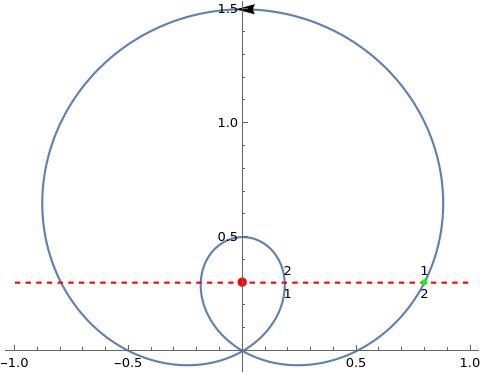
\includegraphics{windingNumber}
        \caption{How to count the winding number}
        \label{fig: Winding Number}
    \end{figure}
\end{definition}
\begin{example}
    Name says it all, winding number counts how many times a curve winds around a point.
    (Positive means anticlockwise winding and negative means clockwise winding.)
    See Figure \ref{fig: Winding Number}.
    Start from the green point (on the side labeled 1), and follow the curve in the direction of the arrow (anticlockwise).
    Once you get to the inner point also labeled 1, it means you've counted one winding.
    Continue from the point inner labeled 2 until you get to the green point (on the side labeled 2).
    You've now counted the second winding.

    Overall, the winding number around the red point is 2.

    If the direction of the arrow were reversed (so that it is clockwise),
    you would've ended up with -2 as the winding number.
\end{example}
\begin{remark}
    The explicit integral representation of the winding number is an application of Cauchy's integral formula to $f(z) \equiv 1$,
    which again I remark is an application of the residue theorem!
\end{remark}
\begin{exercise}
    Prove (or justify) why the explicit form involving the integral should be the winding number (if you are justifying, you could use residue calculus).
\end{exercise}
\begin{exercise}[Cauchy's Integral Formula for Derivatives]
    If $f:U \rightarrow \C$ is holomorphic on open set $U$, then for any $z_0 \in U$,
    $f(z)$ is equal to its Taylor series at $z_0$, and it converges on any open disk
    centered at $z_0$ lying in U,
    and derivatives are given by
    \begin{equation*}
        f^{(n)} (z_0) = \frac{n!}{2\pi i} \int_{\gamma (a,r)} \frac{f(z)}{(z-z_0)^{n+1}} \intd z
    \end{equation*}
\end{exercise}
\begin{remark}
    This implies that ``analytic = holomorphic''!
    They can be used interchangeably!
    This also means \ul{holomorphic functions are infinitely differentiable}.
\end{remark}
\begin{exercise}[Liouville's Theorem]
    Suppose $f:\C \rightarrow \C$ is an entire\footnote{Holomorphic on $\C$} function.
    If $f$ is bounded, then $f$ is a constant function.
\end{exercise}
\begin{remark}
    A part of fundamental theorem of algebra can be proven using Liouville's theorem!
\end{remark}
\begin{example}[Wiener-Hopf Method]
    \textbf{THIS IS ABSOLUTELY OUT OF SCOPE FOR PART A},
    but demonstrates how powerful Liouville's theorem can be!

    Suppose you want to solve the following problem for smooth bounded $f(x)$ for $x \in \R$:
    \begin{equation*}
        \int_{0}^{\infty} K (x-t) f(t) \intd t = f(x) \hspace{1cm} \text{for } x\geq 0
    \end{equation*}
    where $K(x) = e^{-|x|}$ for $x \in \R$.

    \ul{After a bit of trickery\footnote{In a nutshell, one takes (complex) Fourier transform of the entire problem} (in Applied Complex Variables in part C)},
    you end up needing to solve the following for
    $\hat f_{+}$ and $\hat h_{-}$ (or at least one of the two unknown functions):
    \begin{equation*}
        \frac{1-k^2}{k+i} \hat f_{+} (k) = \left( k-i \right) \hat h_{-}(k) \hspace{1cm} \text{for } 0 < \Im (k) < 1
    \end{equation*}
    Wait, you have to solve for $\hat f_{+}$ for $\hat g_{-}$ from a single equation?
    The magic here is that the LHS is holomorphic on $\Im (k) > 0$,
    and the RHS is holomorphic on $\Im (k) < 1$.
    Also from more complicated analysis of the problem, we know that
    $\hat f_{+}(k) = O\left( k^{-1} \right)$ and $\hat h_{-} (k) = O\left( k^{-1} \right)$.

    Define $E(k)$ as
    \begin{equation*}
        E(k) = 
        \begin{cases}
            \frac{1-k^2}{k+i} \hat f_{+} (k) & (\Im (k) > 0) \\
            (k-i) \hat h_{-}(k) & (\Im (k) < 1)
        \end{cases}
    \end{equation*}
    (Note that on the intersection $0 < \Im (k) < 1$, either of the definitions work,
    due to the given problem.)
    $E(k)$ is an entire function by construction, and because $\hat f_{+} (k) = O\left( k^{-1} \right)$ and $\hat h_{-} = O\left( k^{-1} \right)$,
    it is bounded at (complex infinity),
    so \ul{by Liouville's theorem} $E(k) \equiv C$ for some constant $C$.
    Hence, (in the definition of Wiener-Hopf method, $f_{+}$ is defined to be $f_{+}(x) = f(x) \mathbb{I}_{x>0}$, where $\mathbb{I}$ is the indicator function.
    \begin{equation*}
        \hat f_{+}(k) = \frac{C\left( k+i \right)}{1-k^2}
    \end{equation*}
    Taking inverse Fourier transform,
    \begin{equation*}
        f(x) = f_{+} (x) = \frac{C}{2\pi} \int_{\Gamma} \frac{\left( k+i \right)e^{-ikx}}{1-k^2} \intd k
    \end{equation*}
    where $\Gamma$ is a contour from $-\infty + ci$ to $+\infty + ci$ for any $c \in \left( 0,1 \right)$.

\end{example}

It turns out that in most cases, the region at which a function ceases to be holomorphic
are isolated most of the time, and sometimes, not even non-holomorphic even if you haven't defined them!
\begin{exercise}[Riemann's Removable Singularity Theorem]
    Suppose $f:U \setminus \left\{ z_0 \right\} \rightarrow \C$ is holomorphic and bounded near $z_0$,
    then show $f$ extends to a holomorphic function on all of $U$.
\end{exercise}
\begin{example}
    Consider $f(z) = \frac{\sin{z}}{z}$.
    From the definition, it seems like $f(z)$ might not be holomorphic at $z=0$,
    but $f(z)$ is bounded around $z=0$ (since $\lim_{z\rightarrow 0} f(z) = 1$),
    and in a neighbourhood away from $z=0$,
    so by Riemann's removable singularity theorem,
    $f(z)$ is holomorphic at $z=0$.

    Note that if it is holomorphic at $z=0$, then it also means it is infinitely differentiable at $z=0$.
\end{example}
\begin{remark}[General Strategy for Checking Holomorphicity]
    Given $f(z)$,
    \begin{enumerate}
        \item Identify which points might be problematic.
        \item Check boundedness (often via checking if limit exists).
        \item If bounded, then it is definitely holomorphic, otherwise not holomorphic at that point.
    \end{enumerate}
\end{remark}
\begin{exercise}
    \begin{itemize}
        \item Given $f(z) = \frac{\sin{z}}{\cos{z}}$, is it holomorphic at $z=\frac{\pi}{2}$?
        \item What about $f(z) = \frac{\left( z-\frac{\pi}{2} \right)\sin{z}}{\cos{z}}$?
        \item Is $f(z) = \frac{1}{(z+1)^2 (z-1)}$ holomorphic at $z=i$? What about at $z=1$? What about at $z=-1$?
        \item Define branch cut of $\sqrt{z}$ along the positive real axis.
            Determine if $f(z) = \frac{\left( z+i \right) \sqrt{z}}{z}$ is holomorphic at $z=-i$ and $z=i$, and if holomorphic, evaluate at those points.
    \end{itemize}
\end{exercise}

Here is a kind-of converse to Cauchy's theorem.
\begin{theorem}[Morera's Theorem]
    Suppose $f:U \rightarrow \C$ is a continuous function on open $U \subset \C$.
    If for any closed path $\gamma$ in $U$, $\int_{\gamma} f(z) \intd z$,
    then $f$ is holomorphic.
\end{theorem}

\section{Identity Theorem, Isolated Zeros, and Singularities}
I've mentioned it before, but we deal with isolated singularities often,
that is, the isolated points which some function $f$ is not holomorphic.
\begin{definition}[Pole and Order]
    Suppose $f(z)$ is holomorphic on $U \setminus \left\{ a \right\}$ for some $a \in \C$.
    The minimum $n \in \mathbb{Z}^{n \geq 0} \cup \left\{ +\infty \right\}$ such that $\left( z-a \right)^{n} f(z)$ is holomorphic on $U$ is called \textbf{pole} of \textbf{order} $n$ of $f$ at $z=a$.
    \begin{itemize}
        \item If $n = 0$, then we say $a$ is a \textbf{removable singularity}\footnote{You can think of this as not having any singularity at all, in fact; if we have removable singularity, it means we can ``get rid of'' it by analyticity.} as before.
        \item If $n = 1$, then we say $a$ is a \textbf{simple pole}.
        \item If $1 \leq n < \infty$, then we say $a$ is a \textbf{pole of order} $n$.
        \item If $n = \infty$, then we say $a$ is an \textbf{essential singularity}.
    \end{itemize}
\end{definition}
\begin{example}
    \begin{itemize}
        \item $\frac{\sin {z}}{z}$ has a removable singularity at $z=0$.
        \item $\frac{1}{z}$ has a simple pole at $z=0$.
        \item $\frac{1}{z^2}$ has a pole of order 2 at $z=0$.
        \item $\frac{1}{\cos{z}}$ has simple poles at $z = \frac{\pi}{2} \pm n \pi$ for $n \in \mathbb{Z}$.
        \item $e^{\frac{1}{z}}$ has essential singularity at $z = 0$.
    \end{itemize}
\end{example}
\begin{remark}[Determining the Order, Laurent Series, and Residue]
    For \ul{tips on determining the order of a singularity}, refer to \url{https://github.com/pauljoohyunkim/OxfordMathematicsNotesForPoorSouls/blob/main/2nd\%20Year/Metric\%20Spaces\%20and\%20Complex\%20Analysis/Residue\%20Calculus/Computing\_Residue.pdf}.

    But, here are the main points:
    \begin{enumerate}
        \item Identify where the singularities are (in most cases, it is the zeros of the denominator of the functions you are given).
        \item Taylor expand the denominator (and possibly the numerator).
        \item Use the formula $\frac{1}{1-r} = 1 + r + r^2 + \cdots$ for $|r| < 1$ to transform denominator to a multiplication by an infinite series.
    \end{enumerate}
    What you are basically computing is ``Laurent series'' which gives all the info about the order of the pole and residue,
    which will be introduced very shortly.
\end{remark}
\begin{remark}
    The idea of isolated singularity is also very important to residue calculus.
\end{remark}
\begin{theorem}[Identity Theorem]
    Let $U$ be a domain, and $f_1$ and $f_2$ are holomorphic on $U$.
    If $S = \left\{ z \in U | f_1(z) = f_2 (z) \right\}$ has a limit point in $U$,
    then $S = U$, and hence $f_1(z) = f_2 (z)$.
\end{theorem}
\begin{remark}
    In a way, you could think of it as, if two functions $f_1$ and $f_2$ agree on limiting points on a ``dense set'',
    then they must be equal on the domain.

    One could think intuitionistically by noting that if $f$ is holomorphic at $z_0$, then
    $f$ is equal to its Taylor series \ul{in a neighbourhood} around that point.
\end{remark}
\begin{exercise}
    Suppose $f$ has a pole of order $m$ at $z_0$.
    Show that there exists some $r > 0$ such that for all $z \in B\left( z_0, r \right) \setminus\left\{ z_0 \right\}$,
    \begin{equation*}
        f(z) = \sum_{n \geq -m} c_n (z-z_0)^n
    \end{equation*}
    that is,
    $f$ is equal to its \textbf{Laurent series} in any sufficiently small annulus around $z_0$.
    (Hint: What is the definition of a pole of order $m$?)
\end{exercise}
\begin{remark}
    If $f$ has essential singularity at $z_0$, then Laurent series goes from negative infinity to positive infinity:
    \begin{equation*}
        f(z) = \sum_{n = -\infty}^{\infty} c_n (z-z_0)^n
    \end{equation*}
\end{remark}
\begin{definition}[Principal Parts and Residue]
    Given $f$ in its Laurent series around $z_0$,
    \begin{equation*}
        f(z) = \sum_{n = -\infty}^{\infty} c_n (z-z_0)^n
    \end{equation*}
    (where $c_m = 0$ for $m \leq -k-1$ if pole of order $k$)
    the \textbf{principal part} of $f$ at $z_0$ is
    \begin{equation*}
        \sum_{n = -\infty}^{-1} c_n \left( z-z_0 \right)^n
    \end{equation*}
    and \textbf{residue} of $f$ at $z_0$ is
    \begin{equation*}
        \res_{z=z_0} f(z) = c_{-1}
    \end{equation*}
\end{definition}
\begin{remark}
    You might wonder why the principal part and residue are defined this way.

    Principal part is the only part that results in $f$ having a ``singularity'',
    so for singularity analysis, one only needs to look at the principal part.

    Residue is actually really cool.
    Consider counterclockwise integral of $f(z)$ (assume holomorphic in the unit circle except at 0) around the unit circle around $0$.
    \begin{align*}
        \int_{|z| = 1} f(z) \intd z &= \int_{|z| = 1} \sum_{n=-\infty}^{\infty} c_n z^n \intd z\\
        &= \int_{|z| = 1} \frac{c_{-1}}{z} \intd z \\
        &= 2 \pi i \res_{z=0} f(z)
    \end{align*}
    where the second equality comes from Exercise \ref{eg: Taylor Term Circle Integral}.
    This means if you know the residues of $f(z)$ at its singularities,
    then one could compute closed-curve integrals of $f(z)$ easily,
    and this is the motivation for the residue calculus.
\end{remark}
\begin{example}[Computing Residues]
    (As mentioned before)
    For examples of computing residues step-by-step, refer to \url{https://github.com/pauljoohyunkim/OxfordMathematicsNotesForPoorSouls/blob/main/2nd\%20Year/Metric\%20Spaces\%20and\%20Complex\%20Analysis/Residue\%20Calculus/Computing\_Residue.pdf}

    Conceptually, it is important that you recall that you can write $f(z)$ as its
    Laurent series around an annulus centered at its singularity.
\end{example}
\begin{exercise}[Residue of $f / g$]
    Suppose $f,g$ are holomorphic functions and $g$ has a zero at $z_0$.
    Show that
    \begin{equation*}
        \res_{z=z_0} \frac{f(z)}{g(z)} = \frac{f(z_0)}{g'(z_0)}
    \end{equation*}
    (Hint: Obviously, consider Taylor expansion, like I told you!)
\end{exercise}
\begin{exercise}[Residue of pole of order $m$]
    (More general than the previous exercise)
    Suppopse $f$ has a pole of order $m$ at $z_0$.
    Show that
    \begin{equation*}
        \res_{z=z_0} (f) = \lim_{z\rightarrow z_0} \frac{1}{\left( m-1 \right)!} \frac{\intd^{m-1}}{\intd z^{m-1}} \left( \left( z-z_0 \right)^m f(z) \right)
    \end{equation*}
    (Hint: Consider Laurent series of $f$.)
\end{exercise}

\section{Homotopies, Simply-Connected Domains, and Cauchy's Theorem}
\begin{definition}[Homotopy and Simply-Connectedness]
    Suppose that $U$ is an open set in $\C$ and $a,b\in U$,
    and that $\eta:\left[ 0,1 \right] \rightarrow U$,
    $\gamma:\left[ 0,1 \right] \rightarrow U$ are paths in $U$
    such that $\gamma(0) = \eta(0) = a$ and $\gamma(1) = \eta(1) = b$.

    $\gamma$ andd $\eta$ are \textbf{homotopic} if there exists a continuous function $h:\left[ 0,1 \right] \times \left[ 0,1 \right] \rightarrow U$ such that,
    \begin{align*}
        h(0,s) &= a \\
        h(1,s) &= b \\
        h(t,0) &= \gamma(t) \\
        h(t,1) &= \eta(t)
    \end{align*}
    See Figure \ref{fig: Homotopy} for examples of homotopicity and non-homotopicity.
    \begin{figure}[h]
        \centering
        \begin{subfigure}[b]{0.5\textwidth}
            \centering
            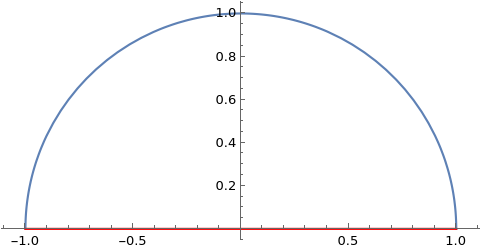
\includegraphics[width=\textwidth]{homotopy1}
            \caption{These two curves are homotopic in $\C$ as you can continuously deform one to get the other.}
        \end{subfigure}
        \hfill
        \centering
        \begin{subfigure}[b]{0.5\textwidth}
            \centering
            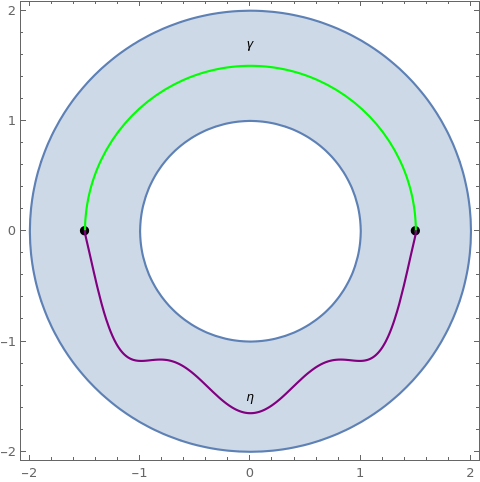
\includegraphics[width=\textwidth]{homotopy2}
            \caption{These two curves are not homotopic in the annulus as you cannot continuously deform one to get the other.}
        \end{subfigure}
        \caption{To talk about homotopy, one must give the two curves and a region.}
        \label{fig: Homotopy}
    \end{figure}
    We say $U$ is \textbf{simply-connected} if two curves in $U$ are always homotopic.
\end{definition}
\begin{exercise}
    You can think of simply-connected regions to be regions without holes
    (though I guess it's an oversimplification.)
\end{exercise}
\begin{exercise}[Deformation Theorem I]
    \label{ex: Deformation Theorem}
    Let $U$ be simply-connected domain.
    Let $f:U \rightarrow \C$ be holomorphic on $U$.
    If $\gamma, \tilde\gamma$ are paths in $U$ from $a \in \C$ to $b \in \C$,
    then
    \begin{equation*}
        \int_{\gamma} f(z) \intd z = \int_{\tilde\gamma} f(z) \intd z
    \end{equation*}
    (Hint: It helps to draw! It becomes basically a one-line argument by the use of Cauchy's theorem.)
\end{exercise}
\begin{exercise}[Deformation Theorem II]
    \label{ex: Deformation Theorem II}
    (Nonexaminable? Maybe? idk)
    For closed curves, there are no ``ends'', so you can deform it how ever you want so long as it does not cross any non-holomorpic region.
\end{exercise}

\section{Argument Principle}
We say function is \textbf{meromorphic} if it is holomorphic except at a few isolated singularities.

Let's start with a simple (verification) exercise.
\begin{exercise}
    Suppose $f:U \rightarrow \C$ is meromorphic and has zero of order $k$ or a pole of order $k$ at $z_0 \in U$.
    Then show that $\frac{f'(z)}{f(z)}$ has a simple pole at $z_0$ with residue $k$ or $-k$ respectively.
\end{exercise}

Here is the statement of the argument principle
\begin{exercise}[Argument Principle]
    Suppose $f:U \rightarrow \C$ is a meromorphic function on $U$.
    Assume $B(a,r) \subset U$.
    Let $N$ denote the number of zeros (counted with multiplicity)
    and $P$ denote the number of poles (counted again with multiplicity)
    of $f$ inside $B(a,r)$,
    and $f$ has neither zeros nor poles on $\partial B(a,r)$, then
    show that
    \begin{equation*}
        N - P = \frac{1}{2\pi i}\int_{\gamma} \frac{f'(z)}{f(z)} \intd z
    \end{equation*}
    where $\gamma$ is a path with image $\partial B (a,r)$.

    Moreover, $N-P$ is also the winding number of the path $\Gamma = f \circ \gamma$.
\end{exercise}
\begin{remark}
    You should now be convinced that you can think of pole as a reverse zero if you have not already\dots
\end{remark}
\begin{remark}
    For understanding of the argument principle,
    I found this resource to be incredibly helpful:
    \url{https://youtu.be/79-ESkh5\_f0}
    Highly recommend the videos by the channel as well for complex analysis to get a grasp of some of the concepts!
\end{remark}

Here is another result proven using argument principle.
\begin{exercise}[Rouch\'e's Theorem]
    Suppose $f,g$ are holomorphic functions on open set $U \subset C$ and
    $\bar B (a,r) \subset U$.
    If $|f(z)| > |g(z)|$ for all $z \in \partial B(a,r)$ then $f,f+g$ both have the same change in argument around $\partial B (a,r)$, and hence the same number of zeros in $B(a,r)$ (counted with multiplicities).
\end{exercise}
\begin{remark}
    Apprently Rouch\'e's theorem is useful for counting number of zeros of a function $f$.
\end{remark}
\begin{example}
    (An example from the lecture note)
    Let $P(z) = z^4 + 5z + 2$. On circle $|z| = 2$, $|z|^4 = 16 > 5.2 + 2 \geq |\underbrace{5z + 2}_{g(z)}|$.
    Then $P-g = z^4$ and $P$ has the same number of roots in $B(0,2)$,
    so by Rouch\'e's theorem, all four roots of $P(z)$ fall in $B(0,2)$.
    Taking $|z|=1$, $|g(z)| \geq 5 - 2 = 3 > |z^4| = 1$, so
    $P(z)$ and $g(z)$ have the same number of roots in $B(0,1)$, so
    $P(z)$ has one root of modulus less than 1, and 3 of modulus between 1 and 2.
\end{example}
Other theorems that sound quite trivial can now be proven:
\begin{exercise}[Open Mapping Theorem]
    Suppose $f:U \rightarrow \C$ is holomorphic and nonconstant on $U$.
    Then for any open set $V \subset U$, $f(V)$ is also open.
\end{exercise}
\begin{exercise}[Inverse Function Theorem]
    Suppose $f:U \rightarrow \C$ be injective and holomorphic, and $f'(z) \neq 0$ for all $z \in U$.
    If $g: f(U) \rightarrow U$ is the inverse of $f$, then
    $g$ is holomorphic, and $g'(w) = \frac{1}{f'(g(w))}$.
\end{exercise}


\section{Residue Theorem}
You are now at the heart of complex analysis!
All the buildup for one of the most important results in complex analysis\dots
I know it's tiring, but this is one of the sections that is almost guaranteed to be on the exam,
and you can actually prepare for it by practice!
\begin{exercise}[Residue Theorem]
    Suppose $U$ is an open set in $\C$ and $\gamma$ is a closed curve whose inside is contained in $U$ (so that $\forall z \not \in U$, $I(\gamma,z) = 0$.)
\end{exercise}
Then if $S \subset U$ is a finite set such that $S \cap \gamma^*$ and $f$ is a holomorphic function on $U \setminus S$,

Here is a very important theorem.
(Don't worry if it looks complicated. In practice, you will be working with very nice functions.)
\begin{equation*}
    \frac{1}{2\pi i} \int_{\gamma} f(z) \intd z = \sum_{a \in S} I \left( \gamma, a \right) \res_{z=a} (f)
\end{equation*}
\begin{remark}
    In most cases, winding number $I(\gamma, a)$ will be 1 (or -1 if you go clockwise), so the RHS in most cases becomes $\pm \sum_{a \in S} \res_{z=a} (f)$
\end{remark}
\begin{remark}
    Explicit form of the winding number, Cauchy's integral formula, and the argument principle can be understood as a case of residue theorem!
    Armed with \ul{residue theorem and deformation theorem} (Exercise \ref{ex: Deformation Theorem}, \ref{ex: Deformation Theorem II}),
    you can compute a vast types of integrals really easily!
\end{remark}
\begin{remark}
    We could've done Example \ref{eg: Taylor Term Circle Integral} using residue theorem really quickly!
\end{remark}
\begin{exercise}
    Verify the following result:
    \begin{equation*}
        \int_{\gamma} \frac{\sin{z}}{\cos{z}} \intd z = 2 \pi i
    \end{equation*}
    where $\gamma$ is a clockwise circular path of radius 0.2 around $\pi/2$
    (Note: Beware of the sign!)
\end{exercise}
\begin{exercise}
    Verify the following result:
    \begin{equation*}
        \int_{\gamma} \frac{1}{\left( z+1 \right)^2 \left( z-1 \right)} \intd z = -\frac{i \pi}{2}
    \end{equation*}
    where $\gamma(t) = -1 + \frac{1}{5} e^{it}$ over $t\in\left[ 0,2\pi \right]$.
\end{exercise}


\subsection{Residue Calculus}
Being able to compute complex integrals very easily means one could now compute real integrals that does not have an easy antiderivative.
\begin{example}
    Suppose we wish to compute
    \begin{equation*}
        \int_{0}^{2\pi} \frac{1}{1+3 \cos^2 (t)} \intd t
    \end{equation*}
    If we consider the path $t \mapsto e^{it}$ (a unit circle),
    and let $z = e^{it}$, and note that
    \begin{equation*}
        \cos{t} = \frac{1}{2} \left( z + \frac{1}{z} \right)
    \end{equation*}
    (since $z$ is on the unit circle)
    we can turn the real integral into complex integral by the transforming the integrand
    \begin{equation*}
        \frac{1}{1+3 \cos^2 (t)} = \frac{1}{1+3 \times \left( \frac{1}{2}\left( z+\frac{1}{z} \right) \right)^2} = \frac{4z^2}{3 + 10z^2 + 3z^4}
    \end{equation*}
    and noting $\intd z = iz \intd t$:
    \begin{equation*}
        \int_{0}^{2\pi} \frac{1}{1+3 \cos^2 (t)} \intd t = \int_\gamma \frac{-4iz}{3+10z^2 + 3z^4} \intd z
    \end{equation*}
    By residue theorem, the complex integral is simply $\pi$, so
    \begin{equation*}
        \int_{0}^{2\pi} \frac{1}{1+3 \cos^2 (t)} \intd t  = \pi
    \end{equation*}
\end{example}
\begin{remark}
    One question you might have is how I came up with the path to be a unit circle.
    Whenever you see an integral involving trig function such as $\sin t$ or $\cos t$, with integration range $\left[ 0,2\pi \right]$ you know that you can write it as some combination of $z, \bar z$, but it is convenient to take the curve to be unit circle so that $\bar z = \frac{1}{z}$, so that we don't have to worry about the conjugate symbol.

    At the end of the day, \ul{it is up to how much you've practiced}.
\end{remark}
\begin{remark}[Some Categorized Examples of Residue Calculus]
    Refer to part C Applied Complex Variables lecture note (\url{https://courses.maths.ox.ac.uk/pluginfile.php/22180/mod_resource/content/1/C5_6LectureNotes.pdf}),
    section 1.9 for some VERY DOABLE examples.
    Note that the entire first section is in fact a highly condensed summary of relevant materials from complex analysis!
\end{remark}
\begin{example}
    Suppose we want to compute
    \begin{equation*}
        I \coloneqq \int_{0}^{\infty} \frac{1}{1+x^2+x^4} \intd x
    \end{equation*}
    Note that I can write this as
    \begin{equation*}
        I = \frac{1}{2} \lim_{R \rightarrow \infty} \int_{-R}^{R} \frac{1}{1+x^2+x^4} \intd x
    \end{equation*}
    It is difficult (if impossible) to get a simple form for the antiderivative of the integrand.
    This means we have to use complex integrals.

    Note that the integral is over the range $[-R, R]$, and we see that at infinity,
    the integrand is like $O\left( z^{-4} \right)$ as $z \rightarrow \infty$ (where $z \in \C$), which seems to indicate that
    the integrand decays at a sufficient rate (and hence be zero at infinity\dots All of this is hand-wavy, but it will make more sense as you practice)

    Consider the following complex integral:
    \begin{equation*}
        \tilde I_R \coloneqq \int_{\gamma_R} \frac{1}{1+z^2+z^4} \intd z 
        = \underbrace{\int_{y_R} \frac{1}{1+z^2+z^4} \intd z}_{\rightarrow 2I} + \int_{b_R} \frac{1}{1+z^2+z^4} \intd z
    \end{equation*}
    where $\gamma_R$ is as shown in Figure \ref{fig: Residue Calculus Contour 1} (concatenation of the yellow and blue contours)
    \begin{figure}[h]
        \centering
        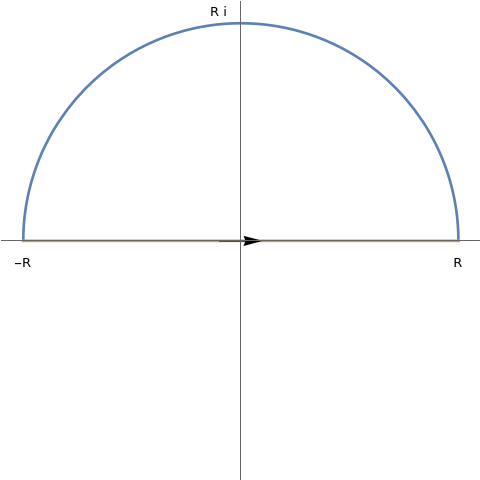
\includegraphics{residueCalculusContour1}
        \caption{Contour for $\tilde I_R$}
        \label{fig: Residue Calculus Contour 1}
    \end{figure}
    and $y_R, b_R$ are yellow and blue paths respectively of the full contour.
    (Note that $\int_{y_R} \frac{1}{1+z^2+z^4} \intd z = \int_{-R}^R \frac{1}{1+x^2+x^4} \intd x$)

    By estimation lemma, the contribution from $b_R$ tends to zero as $R \rightarrow 0$:
    \begin{equation*}
        \left| \int_{b_R} \frac{1}{1+z^2+z^4} \intd z \right|
        \leq \sup_{z \in b_R^*} \left|\frac{1}{1+z^2+z^4}\right| \pi R
        \leq \frac{\pi R}{R^4 - R^2 - 1} \rightarrow 0
    \end{equation*}
    where in the last inequality, I used the (reverse) triangle inequality.
    This implies $\tilde I_R \rightarrow \int_{y_R} \frac{1}{1+z^2+z^4}\intd z$ as $R \rightarrow \infty$.
    This means all we now have to do is to compute $I_R$ using residue theorem, which turns out to be:
    \begin{equation*}
        \tilde I_R = 2 \pi i \left( \res_{z=\omega} \left( \frac{1}{1+z^2+z^4} \right) + \res_{z=\omega^2} \left( \frac{1}{1+z^2+z^4} \right) \right)
        = \pi/\sqrt{3}
    \end{equation*}
    where $\omega\coloneqq e^{i\pi/3}$ 

    Hence, putting it all together,
    \begin{equation*}
        \pi/\sqrt{3} = \lim_{R\rightarrow\infty}\int_{\gamma_R}\frac{1}{1+z^2+z^4} \intd z
    \end{equation*}

    So ultimately,
    \begin{equation*}
        I = \frac{\pi}{2\sqrt{3}}
    \end{equation*}
\end{example}
\begin{remark}[PRO TIP: Behaviour at Infinity]
    \label{rmk: PRO TIP: Behaviour at Infinity}
    (\ul{The outlined technique is only for sanity checks!
    Not to be used in the actual solution!}
The only technique you are given in lecture and hence can be used is the Jordan's lemma. (See Exercise \ref{ex: Jordan's Lemma}))
    If you can infer the behaviour of integral at infinity,
    the whole process of turning real integral into a complex one
    might just become more natural.
    Suppose we have integral $\int_{\Gamma_R} f(z) \intd z$
    such that $f(z) = O\left( \frac{1}{R^n} \right)$,
    and $\Gamma_R$ is a circular arc that ``goes to'' infinity\footnote{Just like the semicircle from the example.} as $R \rightarrow \infty$.

    Bounding the contribution:
    \begin{equation*}
        \left|\int_{\Gamma_R} f(z) \intd z \right|
        \leq \sup_{z \in \Gamma_R^*} |f(z)| \ell(\Gamma_R^*)
        \leq \frac{C_1}{R^n} \left(C_2 R\right)
        =C R^{1-n}
    \end{equation*}
    where
    \begin{itemize}
        \item the first inequality is from estimation lemma.
        \item the second inequality is from the definition of big-O notation and the fact that $\Gamma_R$ is a part of a circle, so we know that $\ell\left( \Gamma_R^* \right) = O\left( R \right)$.
    \end{itemize}
    This means if $n>1$, $\int_{\Gamma_R} f(z) \intd z$ vanishes as $R \rightarrow 0$.
\end{remark}
\begin{example}[Behaviour at Infinity]
    For the following $f(z)$, the integral $\int_{\Gamma_R} f(z) \intd z \rightarrow 0$ as $R \rightarrow \infty$ where $\Gamma_R$ is a part of a circle of radius $R$
    that the following $f(z)$ satisfy $f(z) = O\left( \frac{1}{z^p} \right)$ for some $p>1$.
    \begin{itemize}
        \item $\frac{1}{z+z^2}$
        \item $\frac{1}{z^{3/2}+z^2}$
            \begin{itemize}
                \item $\Gamma_R$ here would have to exclude the branch cut!
            \end{itemize}
        \item $z^ne^{-z}$ for any $n \in \mathbb{Z}$
        \item (WRONG EXAMPLE) $\frac{\sin{z}}{z^2}$
            \begin{itemize}
                \item Note that $|\sin{z}| \leq 1$ is not true in complex analysis!!!
            \end{itemize}
    \end{itemize}
\end{example}

Here is a result that is given in lectures that you ARE allowed to use.
\begin{exercise}[Jordan's Lemma]
    \label{ex: Jordan's Lemma}
    Let $f:\mathbb{H} \rightarrow \C_{\infty}$ be a meromorphic function on
    $\mathbb{H} \coloneqq \left\{ z \in \C | \Im{(z)} > 0 \right\}$.
    Suppose $f(z) \rightarrow 0$ as $z \rightarrow \infty$ in $\mathbb{H}$,
    then if $\gamma_R (t) \coloneqq R e^{it}$ for $t \in \left[ 0, \pi \right]$,
    you have
    \begin{equation*}
        \int_{\gamma_R} f(z) e^{i \alpha z} \intd z \rightarrow 0
    \end{equation*}
    as $R \rightarrow 0$ for any $\alpha > 0$.
\end{exercise}
\begin{remark}
    The pro tip (Remark \ref{rmk: PRO TIP: Behaviour at Infinity})
    covers way more general cases, but you will only need Jordan's lemma in the exam!
\end{remark}

\begin{example}[Integral in the Method of Stationary Phase]
    \textbf{This is material from Part B Waves and Compressible Flow and Part C Perturbation Methods}
    and the exact derivation is not expected in Part A.
    \ul{Howeverm, the relevant bit is the computation of one complex integral.}

    \ul{Method of stationary phase} is a way of approximating an integral of the following form as $x \rightarrow \infty$:
    \begin{equation*}
        I(x) = \int_a^b f(t) e^{i x \psi (t)} \intd t
    \end{equation*}
    where $\psi'(t) \neq 0$ for $a<t<c$ and $c<t<b$ for some $c \in \left[ a,b \right]$, and $\psi''(c) \neq 0$.

    The leading order approximation by method of stationary phase\footnote{In a nutshell, you can derive this by Taylor expanding the integrand at $t = c$ and arguing that the contribution around a small interval around $c$ dominates the contributions from rest of the domain.} turns out to be:
    \begin{equation*}
        I(x) = \underbrace{\frac{f(c) e^{i x \psi(c)}}{x^{1/2}} \int_{-\infty}^{\infty} e^{i s^2 \psi''(c) / 2} \intd s}_{\text{Approximation}} + \underbrace{O\left( \frac{1}{x \epsilon} \right)}_{\text{Correction Term}}
    \end{equation*}
    where the correction term decays as $x \rightarrow \infty$ (enforced by choosing $\epsilon>0$ in some range).
    \ul{To derive the explicit form of the approximation term, one needs to be able to compute:}
    \begin{equation*}
        \tilde I \coloneqq \int_{-\infty}^{\infty} e^{is^2 \psi''(c) / 2} \intd s
    \end{equation*}
    Note that by the ``evenness'' of the integrand, one can write:
    \begin{equation*}
        \tilde I = 2 \int_{0}^{\infty} e^{is^2 \psi''(c)/2} \intd s
    \end{equation*}
    Consider now the following complex integral:
    \begin{equation*}
        J \coloneqq
        \underbrace{
        \int_{R} e^{is^2 \psi''(c)/2} \intd s
    }_{= \tilde I / 2}
        +
        \int_{B} e^{is^2 \psi''(c)/2} \intd s
        -
        \int_{G} e^{is^2 \psi''(c)/2} \intd s
    \end{equation*}
    \begin{figure}[tbp]
        \centering
        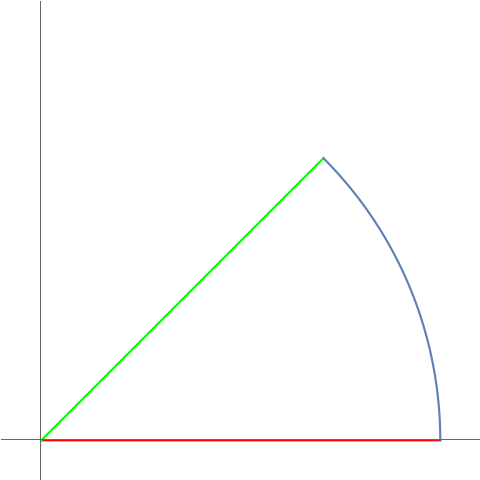
\includegraphics[scale=0.5]{MethodOfStationaryPhase}
        \caption{Integration contour for method of stationary phase for $\psi''(c)>0$. For $\psi''(c)<0$, one could consider the same path reflected across the $x$ axis.}
        \label{fig: Method of Stationary Phase}
    \end{figure}
    where $R, B, G$ refer to the paths specified in red, blue, green in Figure \ref{fig: Method of Stationary Phase}, respectively.
    \footnote{You might wonder \textbf{why this path is chosen};
    it is because as $s$ varies from 0 to infinity,
    the integrand $e^{is^2 \psi''(c)/2}$ ``oscillates'' in some sense,
    and is not an easy integral to evaluate.
    On the other hand, along the $G$ path, by parameterizing it as $s = e^{\pi/4} s$,
    effectively, we now consider a new integrand of the form $e^{-k t^2}$,
    which is a Gaussian integral which we know the value to.
    By relating these two, and the knowledge of complex analysis,
    we can indirectly compute the former integral.
    \ul{Note that this is in fact NOT an obvious choice, and some super clever people thought of it!}
}
    The directions paths are:
    \begin{itemize}
        \item $R$ path goes from the origin to the right infinity.
        \item $B$ path goes around anticlockwise.
        \item $G$ path goes from the origin to infinity at $\pi/4$ angle.
    \end{itemize}
    (Here I have made a deliberate choice to \ul{make $G$ path start from origin rather than going from infinity to origin} for simplicity in dealing with signs later.)
    
    
    \textbf{First},
    Because the integrand does not have any poles inside the closed curve,
    by Cauchy's theorem, $J = 0$.

    \textbf{Second},
    \ul{By Jordan's lemma}, $\int_B e^{is^2 \psi''(c)/2} \intd s \rightarrow 0$ as the radius goes to infinity.

    \textbf{Hence},
    putting these two information,
    we deduce that as radius diverges:
    \begin{equation*}
        2 \times \int_G e^{i s^2 \psi''(c) / 2} \intd s
        \rightarrow 2 \int_{t=0}^{\infty} e^{-\psi''(c)t^2/2} e^{i \pi / 4}\intd t
        =
        \tilde I  
    \end{equation*}
    where the second integral comes from substitution $s = e^{i\pi/4} t$.
    
    We finally have $\tilde I$ in terms of a Gaussian integral.
    I invite you to finish the computation and verify that:
    \begin{equation*}
        I(x) = \frac{\sqrt{2\pi} f(c) e^{ix\psi(c)}e^{i\pi/4}}{x^{1/2} \sqrt{\psi''(c)}} + O \left( \frac{1}{x \epsilon} \right)
    \end{equation*}
\end{example}
\begin{remark}
    In the previous example of method of stationary phase,
    if one wants to be less rigorous (for the intuition's sake),
    one could think that the integral contribution of the arc is nearly zero due to the exponential decay (in the positive upper half plane),
    and think of $G$ path as a ``deformation'' from $R$ curve (noting the homotopicity since no pole in the integrand, and complex infinity is treated as just a point)
    hence by deformation theorem
    \begin{equation*}
        \int_{R} e^{is^2 \psi''(c)/2} \intd s
        =
        \int_{G} e^{is^2 \psi''(c)/2} \intd s
    \end{equation*}
\end{remark}

\subsection{Keyhole Contour: When there is a ``constant-factor'' branch cut}
It is straightforward to compute contour integral if it only involves poles;
just use the residue theorem (and/or deformation theorem) and you are all good.

However, what if you have a branch cut?
The problem here is that, \ul{the branch cut that you define may need to extend to infinity,
which means you might not be able to construct a complex integral with a closed loop
enclosing a branch point.}

The resolution here is to use a closed curve avoiding the branch cut around branch points.
These are called \textbf{keyhole contours}.

\begin{example}
    Suppose you want to compute:
    \begin{equation*}
        I \coloneqq \int_{0}^{\infty} \frac{x^{1/2}}{1+x^2} \intd x
    \end{equation*}
    The intuition should say you should try to consider a complex integral of the form:
    \begin{equation*}
        \tilde I \coloneqq \int_{\Gamma} \frac{z^{1/2}}{1+z^2} \intd z
    \end{equation*}
    where $\Gamma$ is a closed curve to be chosen later.

    Because $z^{1/2}$ is a multifunction, one needs to choose a branch cut.
    For computation of $I$, it involves the contribution of the integrand
    on the domain $\left[ 0, \infty \right)$.
    If one chooses the branch cut along the domain, that is, the positive $x$ axis,
    $z^{1/2} \coloneqq \frac{r}{2} e^{i \theta/2}$ ($\theta \in \left[ 0, 2\pi \right]$) has a \ul{sign difference across the branch cut}\footnote{check this!};
    this is a good thing, since you want to be able to end up with an equation of the form:
    \begin{equation*}
        k \int_{0}^{\infty} \left( Integrand \right) \intd x = \ell
    \end{equation*}
    where $k, \ell$ are some constants.\footnote{This is analogous to using IBP twice to evaluate an integral, where you end up turning the problem into a linear equation.}

    \begin{figure}[tbp]
        \centering
        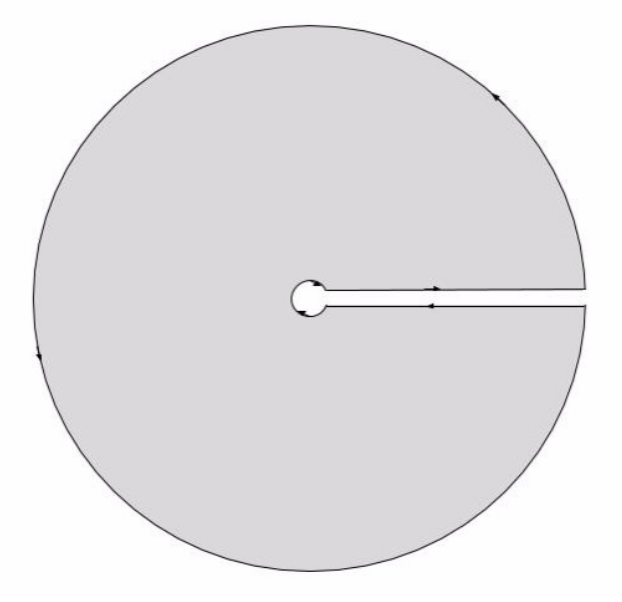
\includegraphics[scale=0.5]{Keyhole}
        \caption{Keyhole contour with branch cut in the positive $x$ axis.}
        \label{fig: Keyhole 1}
    \end{figure}

    Choose $\Gamma$ as Figure \ref{fig: Keyhole 1}.
    Then,
    \begin{equation*}
        \tilde I
        =
        \int_{\gamma_+} \frac{z^{1/2}}{1+z^2} \intd z
        +
        \int_{\gamma_R} \frac{z^{1/2}}{1+z^2} \intd z
        -
        \int_{\gamma_-} \frac{z^{1/2}}{1+z^2} \intd z
        -
        \int_{\gamma_\epsilon} \frac{z^{1/2}}{1+z^2} \intd z
    \end{equation*}
    where
    \begin{itemize}
        \item $\gamma_+$ refers to the straight contour above the positive $x$ axis from ``near origin'' to the right.
            \begin{itemize}
                \item On this contour, $\frac{z^{1/2}}{1+z^2} = \frac{x^{1/2}}{1+x^2}$
            \end{itemize}
        \item $\gamma_R$ is the large anticlockwise arc of radius $R$.
        \item $\gamma_-$ refers to the straight contour below the positive $x$ axis from ``near origin'' to the right.
            \begin{itemize}
                \item On this contour, $\frac{z^{1/2}}{1+z^2} = - \frac{x^{1/2}}{1+x^2}$
            \end{itemize}
        \item $\gamma_\epsilon$ is the small anticlockwise arc of radius $\epsilon$ around the origin.
    \end{itemize}
    (Pay attention to the direction of the contour and all the signs!)
    Considering the values of the $\frac{z^{1/2}}{1+z^2}$ on $\gamma_\pm$,
    note that:
    \begin{equation*}
        \tilde I
        =
        \int_0^{\tilde R} \frac{x^{1/2}}{1+x^2} \intd x
        +
        \int_{\gamma_R} \frac{z^{1/2}}{1+z^2} \intd z
        +
        \int_0^{\tilde R} \frac{x^{1/2}}{1+x^2} \intd x
        -
        \int_{\gamma_\epsilon} \frac{z^{1/2}}{1+z^2} \intd z
    \end{equation*}
    where $\tilde R$ is the $x$ value of the right-end of the $\gamma_{\pm}$,
    which is not important.

    We will be taking the limits as $R \rightarrow \infty$ and $\epsilon \rightarrow 0^+$.

    \textbf{First},
    by residue theorem,
    one can compute $\tilde I = 2\pi i \left( \frac{1}{2} e^{-\pi i / 4} + \frac{1}{2} e^{5 \pi i / 4} \right) = \pi \sqrt{2}$.

    \textbf{Second},
    Note that
    \begin{equation*}
        \left| \int_{\gamma_R} \frac{z^{1/2}}{1+z^2} \intd z \right|
        \leq
        \sup_{z \in \gamma_R} \left|\frac{z^{1/2}}{1 + z^2} \right| \times 2 \pi R
        \rightarrow 0
    \end{equation*}
    where we used estimation lemma, reverse triangle inequality, and sandwich lemma to show that
    the contribution from $\int_{\gamma_R} \frac{z^{1/2}}{1+z^2} \intd z$ decays as $R \rightarrow \infty$.
    \textbf{If you weren't sure if the contribution was zero a priory though},
    read my pro tip at Remark \ref{rmk: PRO TIP: Behaviour at Infinity};
    since $\left|\frac{z^{1/2}}{1 + z^2}\right| \sim \frac{R^{1/2}}{1+R^2} \sim \frac{1}{R^{3/2}} \ll O\left( \frac{1}{R} \right)$ as $R \rightarrow \infty$,
    immediately, you should've known that the contribution is zero.

    \textbf{Third},
    similarly, we note
    \begin{equation*}
        \int_{\gamma_\epsilon} \frac{z^{1/2}}{1+z^2} \intd z
        \leq
        \sup_{z \in \gamma_\epsilon} \left|\frac{z^{1/2}}{1+z^2} \right| 2 \pi \epsilon
        \rightarrow 0
    \end{equation*}
    so again, you get no contribution from this integral\footnote{I haven't thought much into if the trick in Remark \ref{rmk: PRO TIP: Behaviour at Infinity} could work with curve going to zero, but it is worth investigating on your own I guess\dots} in the limit $\epsilon \rightarrow 0$.

    \textbf{Hence},
    putting all these together,
    we deduce
    \begin{equation*}
        2 \int_{0}^{\infty} \frac{x^{1/2}}{1 + x^2} \intd x = \pi \sqrt{2}
    \end{equation*},
    so we get
    \begin{equation*}
        \int_{0}^{\infty}\frac{x^{1/2}}{1 + x^2} \intd x =\frac{\pi}{\sqrt{2}}
    \end{equation*}
\end{example}
\begin{remark}
    The fact that there was a factor (of negative one) difference across the branch cut is what allowed us to use the keyhole contour!
\end{remark}

\begin{example}
    Let's go through the computation of the followwing integral quickly!
    \begin{equation*}
        I \coloneqq \int_{0}^{\infty} \frac{x^{1/2} \log x}{\left( 1+x \right)^2} \intd x
    \end{equation*}
    Remember from discussion of branch cuts of $\log z$ that it doesn't have a constant factor difference across the branch cuts, but a constant addition across the branch cuts;
    this is not a good thing, as it's like using IBP twice and accidentally removing the integral you needed to compute\dots
    Fortunately, in this case, $z^{1/2}$ also provides branch cut, which has a factor difference.

    Using the same keyhole contour (Figure \ref{fig: Keyhole 1}),
    define
    \begin{equation*}
        \tilde I \coloneqq
        \int_{\gamma_+} \frac{z^{1/2} \log z}{\left( 1+z \right)^2} \intd z
        +
        \int_{\gamma_R} \frac{z^{1/2} \log z}{\left( 1+z \right)^2} \intd z
        -
        \int_{\gamma_-} \frac{z^{1/2} \log z}{\left( 1+z \right)^2} \intd z
        -
        \int_{\gamma_\epsilon} \frac{z^{1/2} \log z}{\left( 1+z \right)^2} \intd z
    \end{equation*}

    \textbf{First},
    Note that $\frac{z^{1/2} \log z}{\left( 1+z \right)^2} = \pm \frac{x^{1/2} \log x}{\left( 1+x \right)^2}$ on $\gamma_{\pm}$.

    \textbf{Second},
    Because as $R \rightarrow \infty$,
    \begin{equation*}
        \left| \frac{z^{1/2} \log z}{\left( 1+z \right)^2} \right|
        \sim
        \frac{R^{1/2} \log R}{ R^2}
    \end{equation*}
    by Remark \ref{rmk: PRO TIP: Behaviour at Infinity},
    contribution from $\gamma_R$ is zero.

    \textbf{Third},
    similarly,
    \begin{equation*}
        \int_{\gamma_\epsilon} \frac{z^{1/2} \log z}{\left( 1+z \right)^2} \intd z
        \leq
        \sup_{z \in \gamma_{\epsilon}} \left|\frac{z^{1/2} \log z}{\left( 1+z \right)^2}\right| 2\pi \epsilon
        \rightarrow 0
    \end{equation*}
    so no contribution from $\gamma_\epsilon$.\footnote{For those who want to see in more detail as to showing the limit going to zero, it might be helpful to note that $\epsilon \sqrt{\epsilon} \log \epsilon = \sqrt{\epsilon} \frac{\log \epsilon}{1/\epsilon}$, and use l'H\^opital on $\frac{\log \epsilon}{1/\epsilon}$.}

    \textbf{Fourth}
    computing $\tilde I$ directly using the residue theorem,
    \begin{equation*}
        \tilde I = \pi^2 + 2\pi
    \end{equation*}

    \textbf{Hence},
    putting all the info together (taking real part)
    deduce
    \begin{equation*}
        I = \pi
    \end{equation*}

    As a byproduct, by taking imaginary part instead, you also deduce
    \begin{equation*}
        \int_{0}^{\infty} \frac{\sqrt{x}}{\left( 1+x \right)^2} \intd x = \pi / 2
    \end{equation*}
\end{example}

%\begin{example}[Sine Integral]
%    Consider the following integral:
%    \begin{equation*}
%        I \coloneqq \int_{-\infty}^{\infty} \frac{\sin{x}}{x} \intd x
%    \end{equation*}
%    Again consider a similar contour to Figure \ref{fig: Residue Calculus Contour 1} and the following integral (yellow and blue contour are denoted by $y_R, b_R$ respectively)
%    \begin{equation*}
%        \tilde I_R \coloneqq \underbrace{\int_{y_R} \frac{\sin{z}}{z} \intd z}_{\int_{-R}^R \frac{\sin{x}}{x} \intd x} + \int_{b_R} \frac{\sin{z}}{z}\intd z
%    \end{equation*}
%\end{example}
\end{document}


